\section{Results}\label{sec:results}

\subsection{Calibration: the evaluator supports a mature $\pi_{0.5}$}
The published $\pi_{0.5}$ checkpoint obtains \piRTPublic\% on the same six-task,
four-seed bridge (941/1,200 successes): 93.0 hammer, 96.5 ranking-RGB, 64.0
ranking-size, 53.5 handover, 93.5 Stack-2, and 70.0 Stack-3.  This result is an
evaluator calibration, not a matched baseline, because its training mixture and
recipe differ.  The calibration nevertheless shows that the pilot A0 score is mainly
a policy-training issue rather than a globally broken evaluation bridge.

\subsection{Legacy matched pilot: useful signal, insufficient baseline}
Table~\ref{tab:pi05rt} reports the completed legacy pilot.  Every conditioned
method improves its six-task macro over A0.  A2-Abs gains 13.25 points and A3
gains \piRTAThreeVsZero{} points.  However, the absolute success levels remain
far below the public calibration, each row has one training seed, and A3 exceeds
A2-Abs by only \piRTAThreeVsAbs{} points.  We therefore use this result to choose
the confirmatory arms, not as the final MINT-VLA performance claim.

\begin{table}[H]
\centering\small
\caption{Legacy matched $\pi_{0.5}$ RoboTwin pilot: joint-delta actions,
quantile normalization, batch 64, 20k updates.  Each cell averages 200 accepted
episodes; each row has one training seed.}
\resizebox{\linewidth}{!}{%
\begin{tabular}{lrrrrrrr}
\toprule
Method & Hammer & Rank RGB & Rank size & Handover & Stack-3 & Stack-2 & Macro \\
\midrule
A0: no hint & 70.0 & 50.5 & 24.0 & 9.0 & 17.5 & 42.0 & \piRTAZero \\
A1: external absolute & 79.5 & 52.5 & 24.5 & 5.5 & 22.0 & 63.0 & \piRTAOne \\
A2: offline absolute & 78.0 & 65.0 & 30.5 & 19.5 & 30.5 & 69.0 & \piRTATwoAbs \\
A2: offline residual & 76.5 & 52.5 & 34.5 & 18.0 & 25.0 & 56.5 & \piRTATwoResid \\
A3: MINT-VLA current-encoder & 66.0 & 70.5 & 25.5 & 26.0 & 35.5 & 74.0 & \piRTAThree \\
\bottomrule
\end{tabular}}
\label{tab:pi05rt}
\end{table}

The task profile is heterogeneous (Fig.~\ref{fig:pi05tasks}).  A3 improves
ranking-RGB, handover, and stacking but loses on hammer and ranking-size versus
A2-Abs.  Offline residualization is 4.92 points below offline absolute, so
``more change-focused'' is not equivalent to ``more useful as a policy token.''
The A2-to-A3 contrast further changes target computation, predictor capacity, auxiliary
loss, and the injected value; it motivates Q3 but does not identify which factor
caused the difference.

\begin{figure}[H]
  \centering
  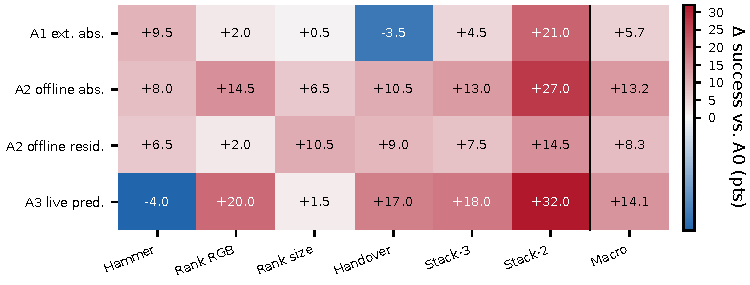
\includegraphics[width=0.88\linewidth]{figures/fig2_redundancy.pdf}
  \caption{Legacy-pilot task deltas relative to A0.  Each cell contains 200
  accepted episodes from one trained checkpoint.  The methods shift
  gains across tasks; none dominates every task.}
  \label{fig:pi05tasks}
\end{figure}

\subsection{The corrected matched comparison is pending}
The corrected A0/A2-Abs/A3 matrix is the primary missing result.  Table
\ref{tab:confirmatory} is intentionally reserved so that pilot numbers cannot
silently become the final baseline.

\begin{table}[H]
\centering\small
\caption{Confirmatory public-recipe RoboTwin matrix.  Report mean and interval
over independent training seeds, plus the full task breakdown.}
\begin{tabular}{lrrr}
\toprule
Method & Train seeds & Six-task macro & $\Delta$ vs. A0 \\
\midrule
A0 no hint & \exptodoid{T0,T2} & \exptodoid{T0,T2} & -- \\
A2 offline absolute & \exptodoid{T1--T2} & \exptodoid{T1--T2} & \exptodoid{T1--T2} \\
A3 MINT-VLA current-encoder & \exptodoid{T1--T2} & \exptodoid{T1--T2} & \exptodoid{T1--T2} \\
\bottomrule
\end{tabular}
\label{tab:confirmatory}
\end{table}

\subsection{The visual token helps, but its predicted future content does not yet}
The five completed A2 conditions do not show that predicted future content
improves control on the
three selected tasks.  Correct, current-state, zero, feature-permuted, and
cross-task content obtain 70.67, 71.00, 67.17, 71.50, and 71.67\% over 600
episodes.  A nonzero visual token helps relative to removing the token, but the
correct prediction is not better than any structured nonzero replacement in
aggregate.  The task profile differs: correct/current/zero are
78.0/73.0/69.5\% on hammer, 65.0/68.5/62.0\% on ranking-RGB, and
69.0/71.5/70.0\% on Stack-2.  Across 179 matched hammer scenes, correct beats
zero in 38 discordant cases and loses in 22 (exact two-sided McNemar
$p{=}0.0519$, before multiplicity correction).  This evidence supports visual
token input but not a general benefit from predicted milestone content.

\begin{table}[H]
\centering\small
\caption{Fixed-checkpoint content intervention.  Final cells use identical
accepted scenes and Holm-adjusted paired tests.}
\begin{tabular}{lrrrrr}
\toprule
Checkpoint & Correct & Current & Zero & Permuted & Cross-task \\
\midrule
A2-Abs & 70.67$^\dagger$ & 71.00$^\dagger$ & 67.17$^\dagger$ & 71.50$^\dagger$ & 71.67$^\dagger$ \\
A3 & 70.17$^\dagger$ & 70.50$^\dagger$ & \exptodoid{E1} & \exptodoid{E1} & \exptodoid{E1} \\
\bottomrule
\end{tabular}
\label{tab:pi05content}
\end{table}
\noindent\footnotesize{$^\dagger$Three-task aggregate over 600 episodes; not
directly comparable to the six-task pilot macro.}\normalsize
\exptodo{E1}{Add within-task instance shuffling for A2; finish A3 zero,
permuted, and cross-task conditions; replace aggregate comparisons with
matched-scene discordant counts and Holm-adjusted tests.}

\subsection{The pilot does not isolate the effect of target recomputation}
No completed comparison holds capacity, target, loss, and injected value fixed
while changing only how the target feature is computed.  Likewise, the current pilot does not
separate forward conditioning from auxiliary representation shaping.
The current evidence therefore supports A3 as an unfactorized
combined integration design, but does not isolate current-encoder target recomputation or residual
parameterization as its cause.

The remaining training matrix tests saved versus recomputed target features,
direct-absolute versus residual-parameterized prediction, auxiliary-only,
prefix-only, detached-current, fixed-horizon, random-future, terminal-frame,
and oracle-milestone controls.
\exptodo{T3}{Populate the factorized mechanism matrix with newly trained,
parameter-matched controls and replicate every claim-bearing contrast.}

\subsection{Task scope and optimization robustness remain unresolved}
The legacy simulator seeds quantify rollout variation around one trained
checkpoint, not optimization variance.  The ordered-construction hypothesis is
also post hoc: on Stack-2/3, legacy A3 averages \piRTStackAThree\% versus
\piRTStackAZero\% for A0, but the public unconditioned checkpoint already
reaches \piRTStackPublic\%.  This may reflect useful stage structure, baseline
room for improvement, or both.  We will make a task-specific claim only if the direction
replicates on predeclared block and bowl stacking, beats a fixed-horizon target
encoded by the current policy, and differs from reactive/contact and geometric control
tasks.

Independent training seeds, matched mature-initialization transfer, and the
predeclared task panel remain pending.  Exact parameter counts and static
predictor FLOPs are reported in the appendix; paired memory and latency
measurements will accompany the confirmatory checkpoints.
\exptodo{T4--T5,E2}{Populate the predeclared scope, mature-transfer, and paired
deployment-cost results.}

\subsection{Use with a second VLA architecture remains to be tested}
The current RoboTwin experiment instantiates MINT-VLA only on $\pi_{0.5}$.  It
tests the one-token prefix implementation, not its use with another VLA
architecture.  A matched experiment on a second VLA is required before the
paper claims evidence beyond the $\pi_{0.5}$ implementation.
\exptodo{T6}{Add a matched second-VLA baseline and MINT-VLA result using the same
milestone construction and evaluation protocol.}

\subsection{Supporting boundary diagnostics}
LaWAM interventions show why Q2 is necessary: correct hints are not reliably
better than zero, instance-shuffled, or cross-task hints, and the former ``no-WM'' arm
inherits WM-aware pretraining and current DINO conditioning.  It is therefore
named \emph{LaWAM-init/Future-off} and used only to diagnose downstream
integration.  LIBERO is similarly auxiliary: its near-saturated four-suite
aggregate is neutral to negative under milestone conditioning.  Full tables
and multiplicity-aware analyses belong in Appendix~\ref{sec:appendix}; neither
diagnostic substitutes for the missing $\pi_{0.5}$ gates.
